\section{Results}
\label{sec:results}
In this section, we show the outcomes of the implemented system architecture, facial and vocal emotion recognition described in the Method chapter and resulting in our overall tool.

\subsection{Experiment Environment \& Testing Setup}
\label{subsec:results_experiment_environment_and_testing_setup}
We set our experiment during a virtual seminar “Collaborative Innovation Networks” (COINs) in the summer semester 2021, held by Prof. Peter Gloor (MIT). The seminar consisted of 23 students from the Universities of Cologne, Bamberg and Lucerne and 3 instructors. All students formed in total 6 teams with three to five participants working on complex subject related and practical topics. Due to the currentstill present global Covid-19 pandemic and an agile project management, every team presented in weekly and bi-weekly sprintshad to present around every two weeks their current status in a virtual Zoom meeting. In each Virtual Status Meeting, every group had to update in ca. 10 min their project goals, present their progress, results or plans  of the last and next iteration, give an output from the retrospective and ask for support by problems or questions.

Since our prototype Moody was not ready for use right at the first meeting and still needed to be developed to track emotions, we were only able to ask the other groups to use our Moody Tracker from the third meeting onwards. For this purpose, we wrote a short usage guide within the invitation before the meeting, so that each group could activate the tracker during their presentation. Therefore, in addition to the usage instructions, we asked the other teams to generate a feedback link via our website (\url{www.moody.digital}) after their presentation and share it with the other meeting participants.

The underlying intention here was primarily receiving instant feedback about our application in real-world usage. This made continuous testing possible, which enabled us to constantly work on errors and bugs reported by the users in each status meeting. Also, we had the chance to quickly collect subjective ratings about the perceived quality of each presentation and compare it to the tracked emotion data. The focus of this paper lies neither in statistically analyzing the correlation nor the causality between experienced emotionality of the audience and the presentation quality, but we had the chance to cursorily analyze the first insights.

Exemplarily we present the following screenshot of our status presentation on the 6th July 2021. With this recording we found that our last presentator on that day seemed to speak rather sad than happy. He was able to use this information for the next presentation in order to increase his positive emotion-transmissions via voice. Additionally, we have seen that the faces and voices were interpreted mainly neutrally, because of the formal and informative character of the presentations. This aligns to our expectations and indicates that the models are predicting correctly.

\begin{figure}
\centering
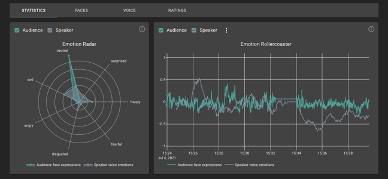
\includegraphics[width=1\textwidth]{assets/moody_statistics_screenshot.png}
\caption{Caption}
\label{fig:moody_statistics_screenshot}
\end{figure}

\subsection{Face Emotion Recognition}
\label{subsec:results_face_emotion_recognition}
Since we adopt the pre-developed \texttt{faceapi.js} and its two underlying models for the face detection and expression recognition, we do not want to focus in this chapter on presenting the resulting metrics and accuracies. Instead we briefly show that we implemented the API correctly in our tool and how it works. The following picture illustrates the presenter's view of the detected faces and their current emotions, when he clicks on the Tab “Faces” while the emotion tracking is running. It seems that the model identifies the emotionalities expressed by the faces correctly.

\begin{figure}
\centering
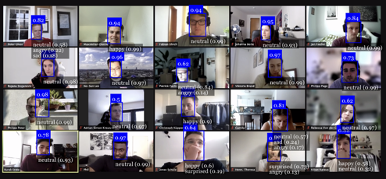
\includegraphics[width=1\textwidth]{assets/moody_faces_screenshot.png}
\caption{Caption}
\label{fig:moody_faces_screenshot}
\end{figure}

The models receive every second a freeze frame from the videoconference window with all participants’ cameras and calculate every second the probabilities for the current face emotion per person respectively per detected face. The probabilities are shown as values between 0 and 1. Exemplarily ``happy (0.8)'' and ``neutral (0.2)'' mean that the particular face looks like 80\% happy and smiling and 20\% neutral. paul ekman emotions...
 if a face 99\% smiles and looks happy. Every emotion from. The formula 
formel:
\begin{itemize}
\item score zusammensetzung: https://github.com/COINS-SS21/moody/blob/main/src/meetings/speakerVoiceEmotionUtils.ts, der score ist pro person und dann noch der durchscnitt von allen teilnehemern
\end{itemize}

\subsection{Vocal Emotion Recognition}
\label{subsec:results_vocal_emotion_recognition}
Since the AlexNet was trained on the four different sets of data (RAVEDESS, EMO-DB, TESS, JL-Corpus) to get as much variety as possible, the accuracy of the model was about 87.17\% (cf. Figure \ref{fig:Accuracy by Epoch}). 

\begin{figure}
\centering
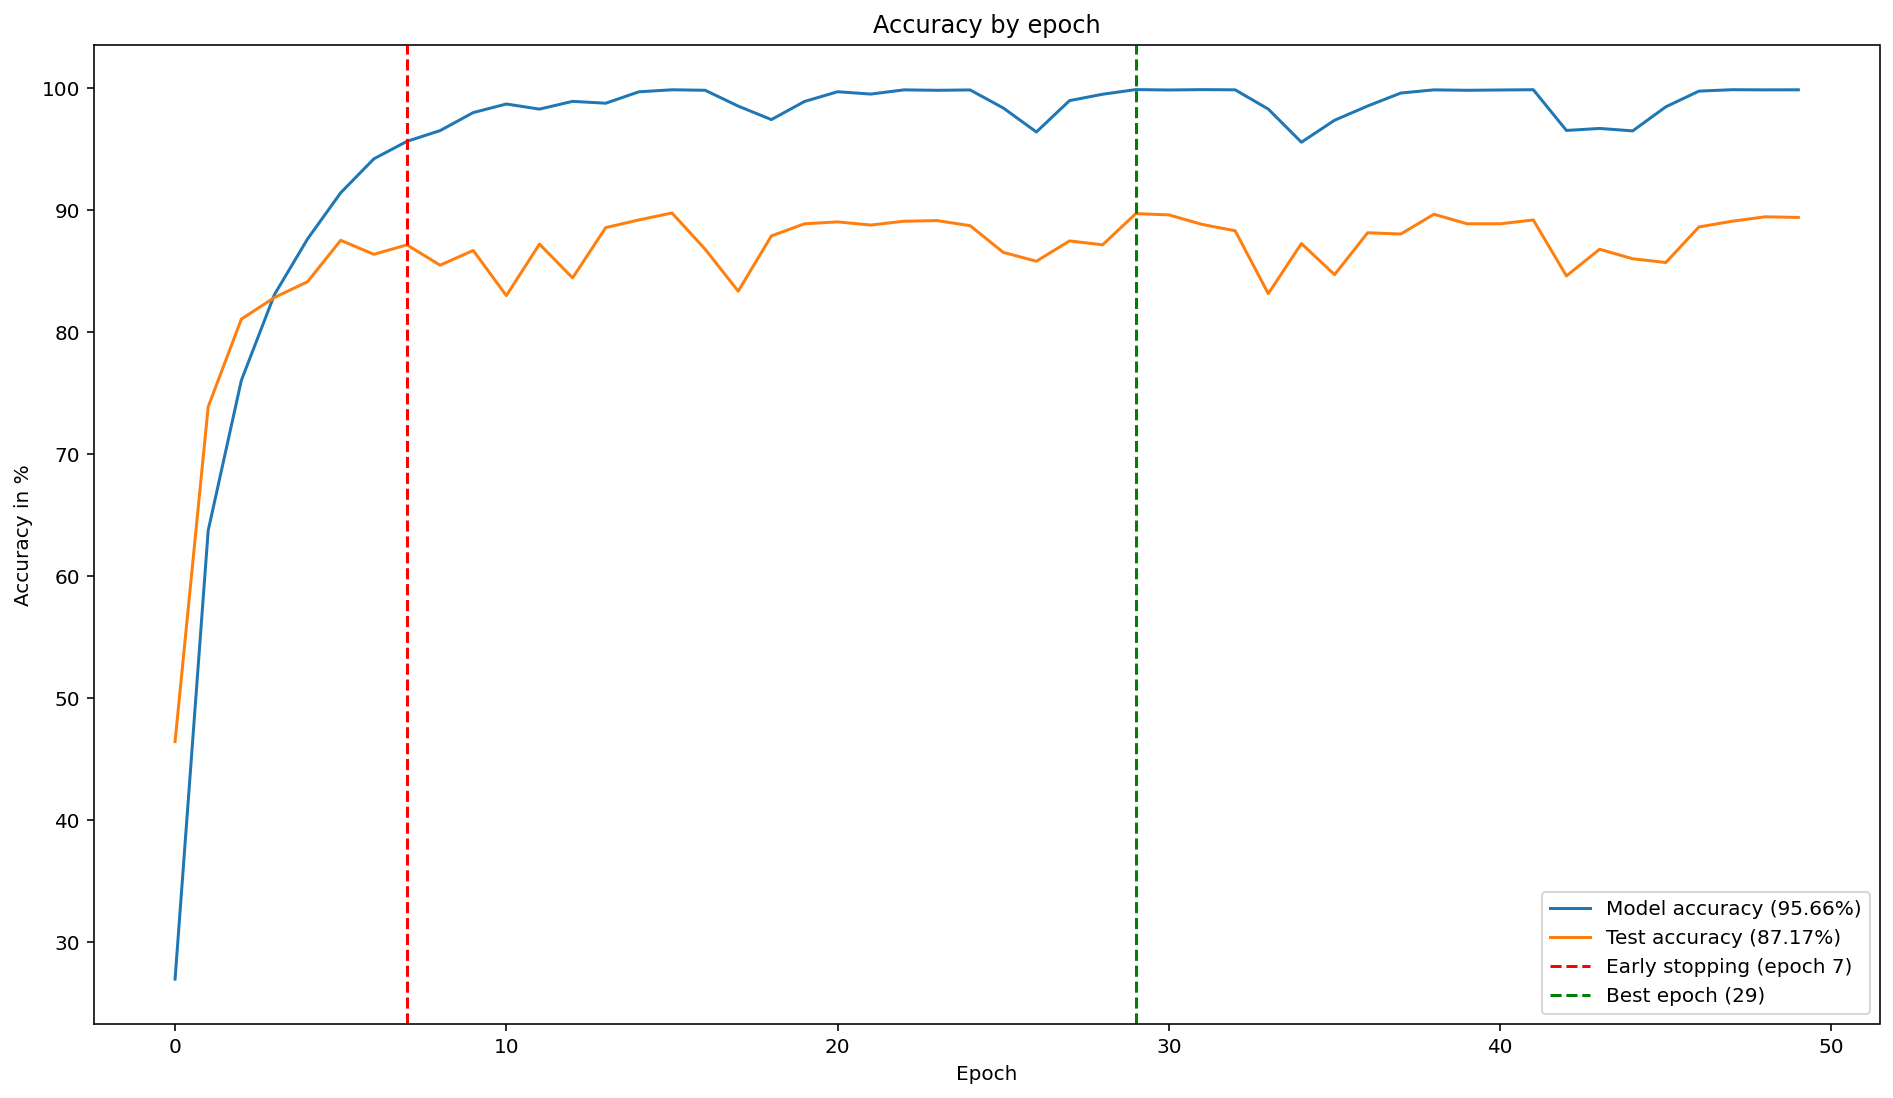
\includegraphics[width=1\textwidth]{assets/alexnet_accuracy.png}
\caption{Accuracy by Epoch}
\label{fig:Accuracy by Epoch}
\end{figure}

To get the best possible result, early stopping was included. This was best at the eighth epoch, as the loss did not change much there either (cf. Figure \ref{fig:CrossEntryLoss by Epoch}).
\newpage
\begin{figure}[h]
\centering
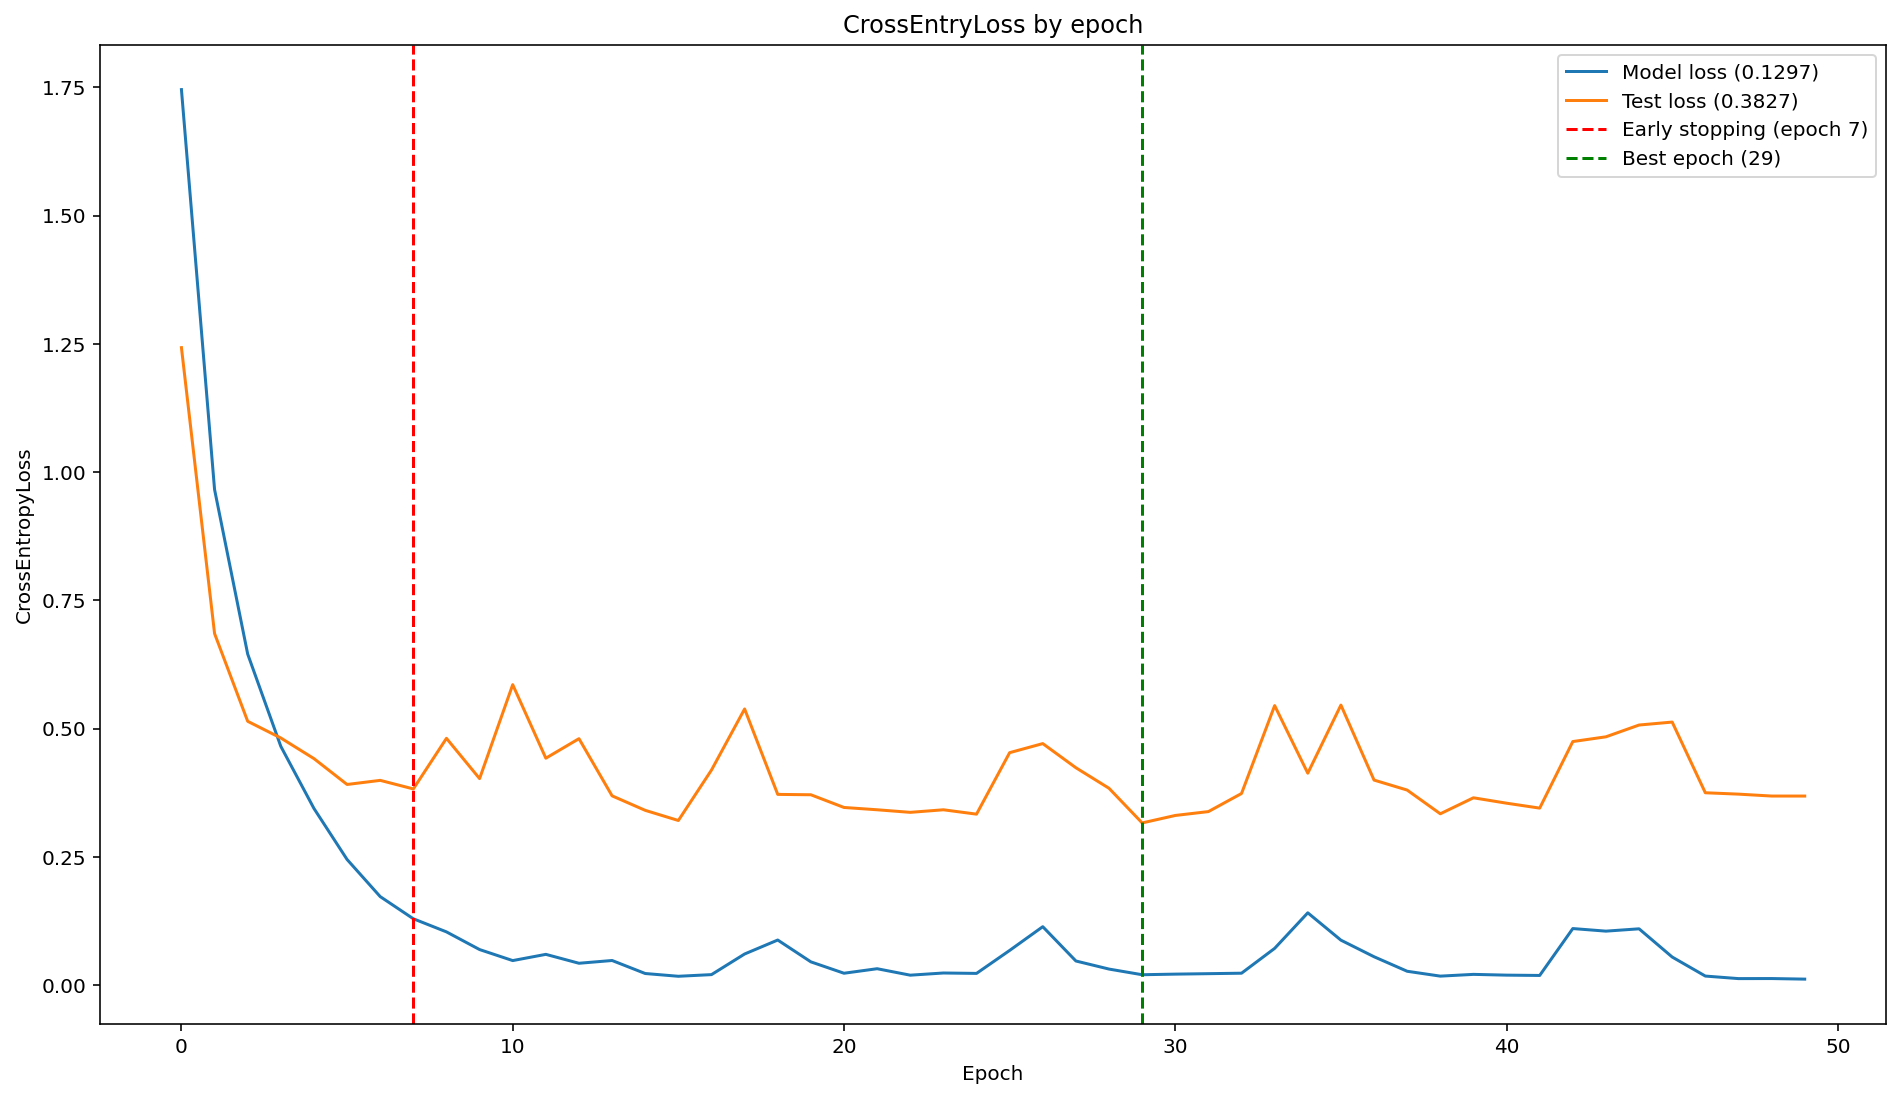
\includegraphics[width=1\textwidth]{assets/alexnet_loss.png}
\caption{Cross Entry Loss by Epoch}
\label{fig:CrossEntryLoss by Epoch}
\end{figure}

The difference to the Res-Net model, apart from minor differences in accuracy, was only the size of the model. The AlexNet has a size of 32.3 MB, whereas the Res-Net has 59.6 MB, almost twice as large. Since the data model is reloaded in the browser every time the voice emotion model is used, which takes up time as well as memory, we finally decided to use the AlexNet. It has a very good accuracy and a small memory size, which is good for everyday use.

\begin{figure}[h]
\centering
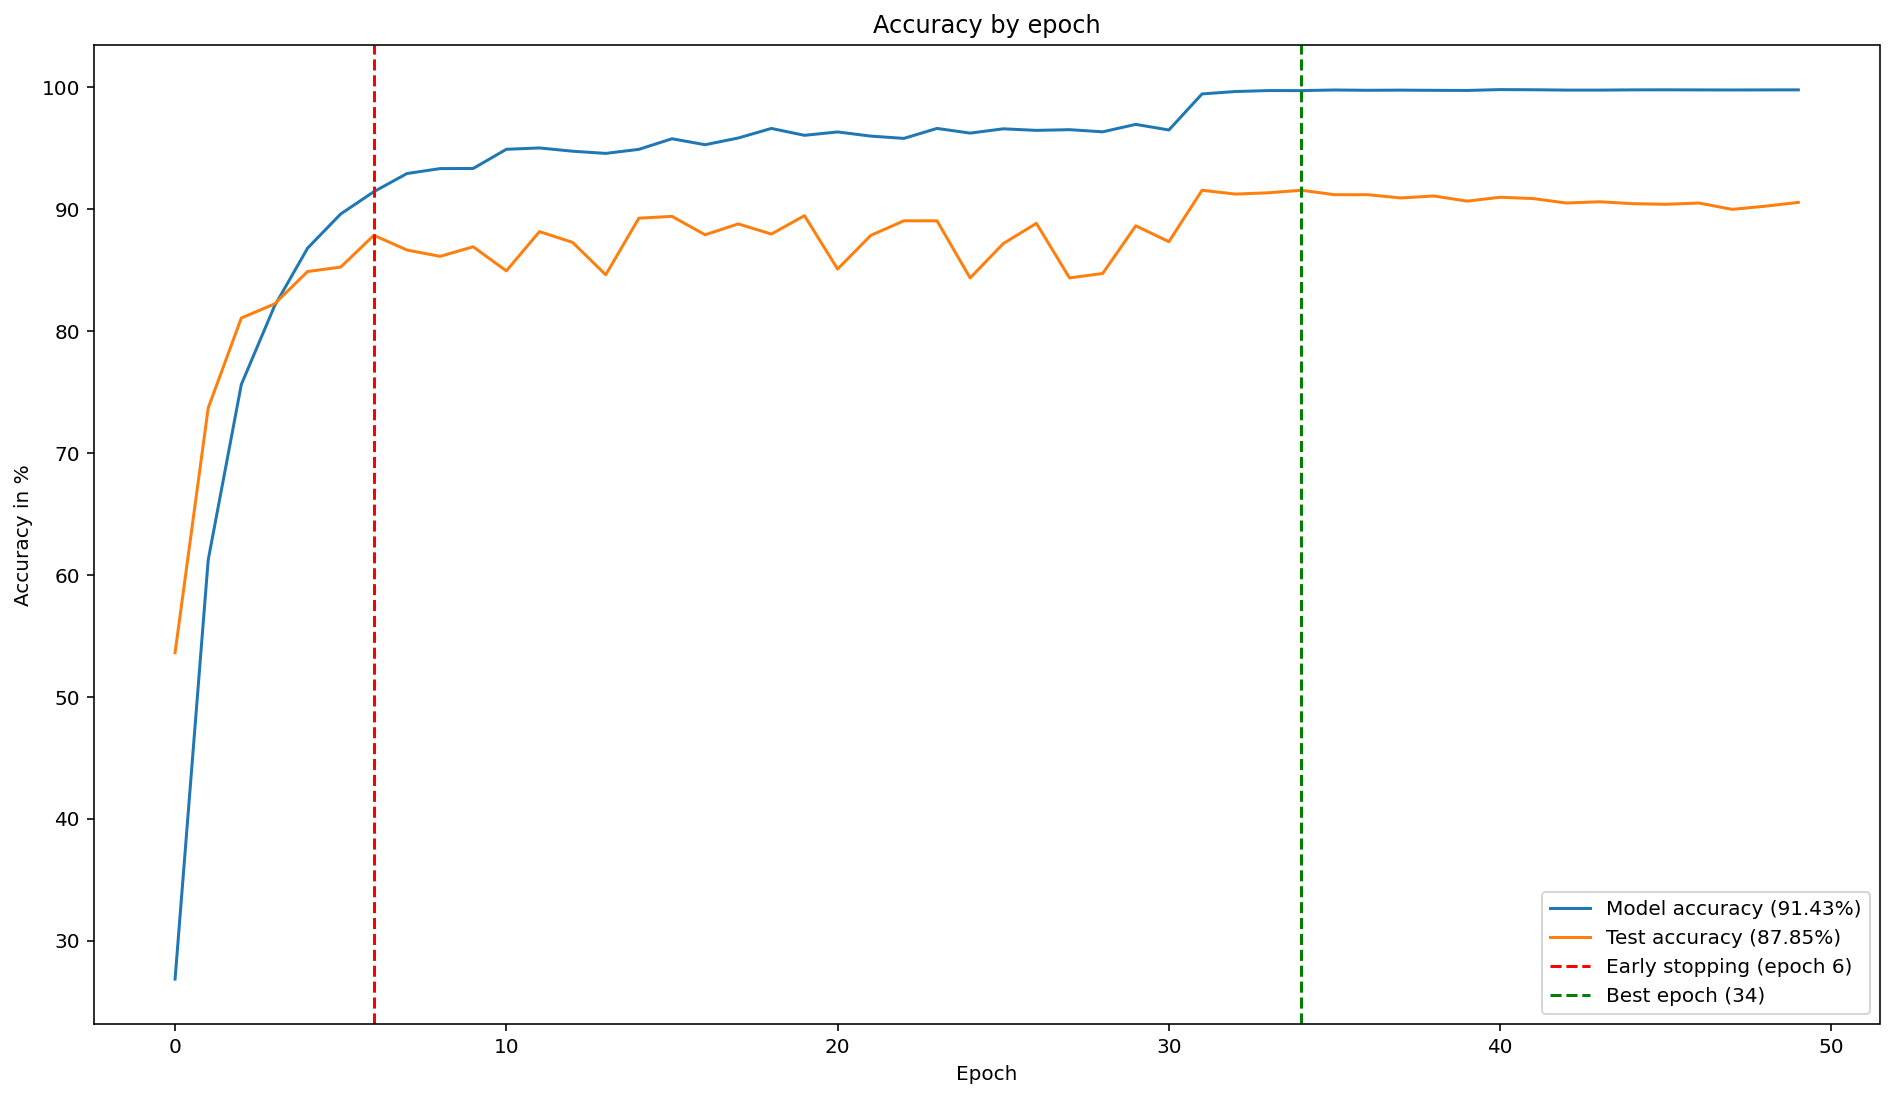
\includegraphics[width=1\textwidth]{assets/resnet_accuracy.png}
\caption{Res-Net Accuracy}
\label{fig:resnet_accuracy}
\end{figure}

Finally, the confusion matrix shows that our model has fairly high prediction values and very low deviations for all emotions (cf. Figure \ref{fig:alexnet_confusion_matrix}).

\begin{figure}[h]
\centering
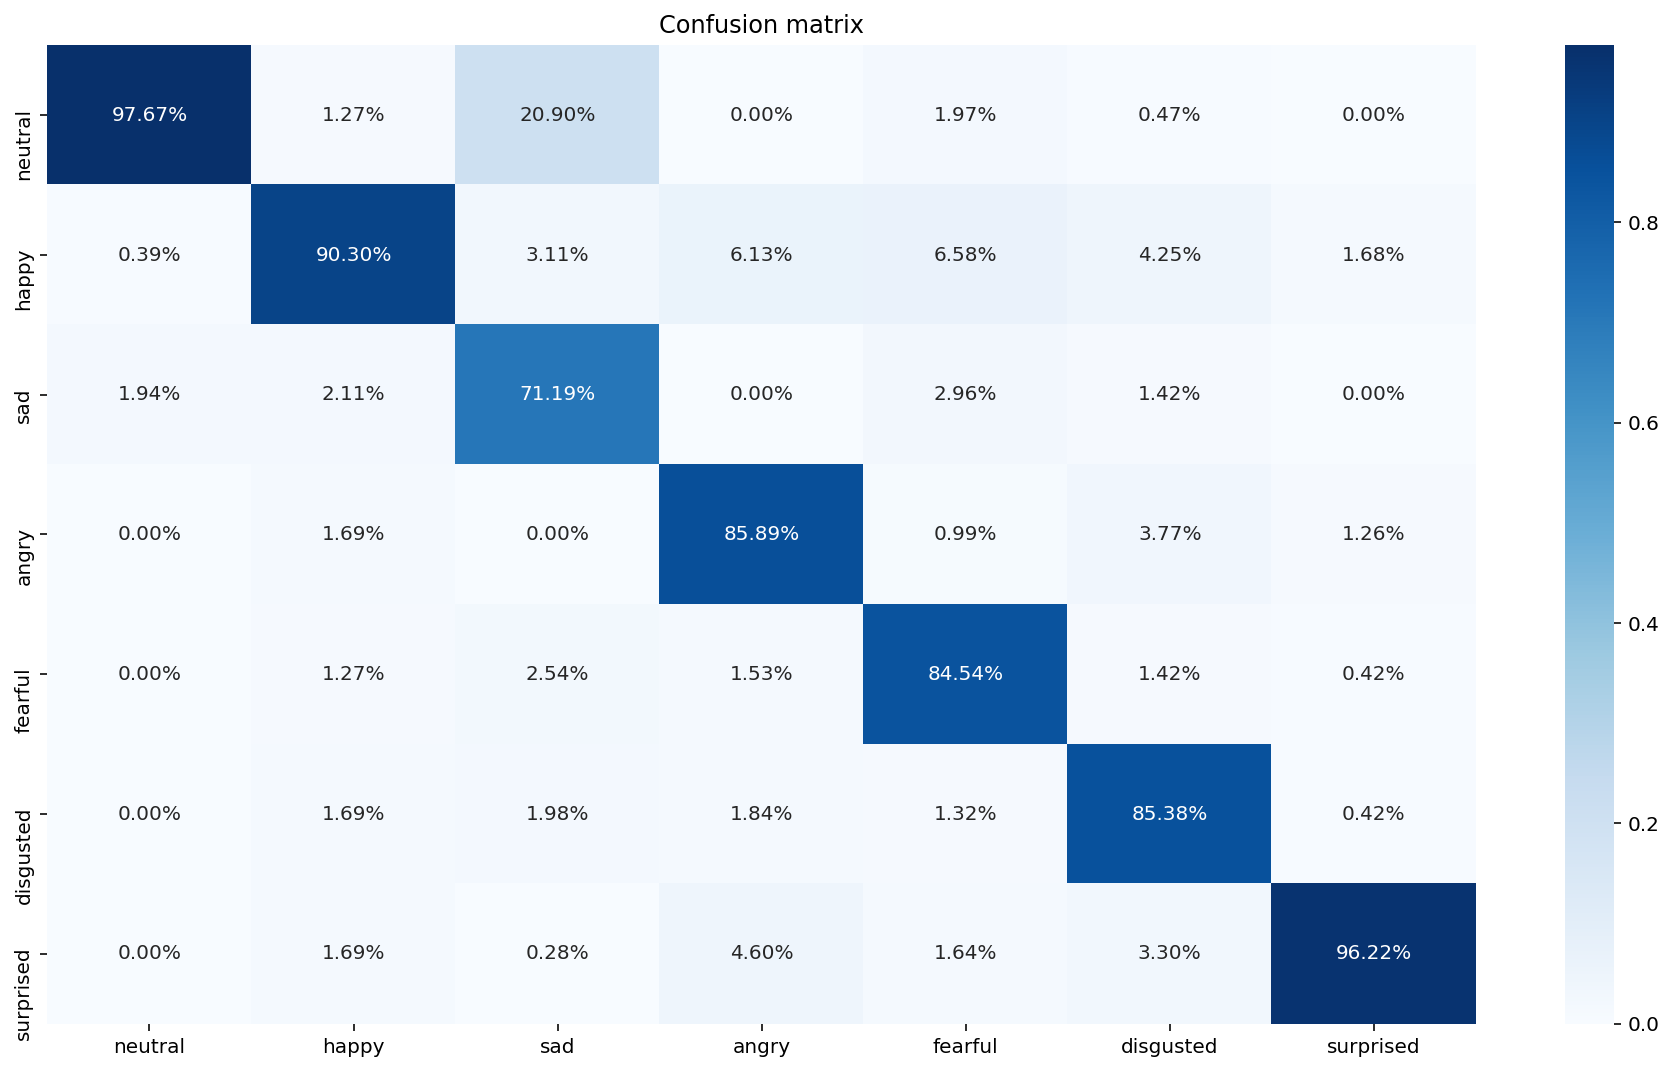
\includegraphics[width=1\textwidth]{assets/alexnet_confusion_matrix.png}
\caption{AlexNet Confusion Matrix}
\label{fig:alexnet_confusion_matrix}
\end{figure}

The voice emotion model can be activated optionally at any time during a meeting. It can be added during any meeting or just at the beginning of the meeting and will be then downloaded through the browser. During the meeting, in addition to the emotion roller-coaster, the voice emotions can also be determined at the current time. A time span of 2.1 seconds is always taken to track the current emotion, which is delivering a good prediction of the emotion at that moment. At the end of the meeting a moving average can be calculated, looking at all the voice emotion tracked in that meeting, to get the most valuable and usable result.  
